\documentclass{source/Paper}
\usepackage{chngcntr}
\setmainfont{SimSun} % 设置主字体为宋体
% \counterwithin{footnote}{page} % 每页重置脚注计数器
\usepackage{perpage}
\MakePerPage{footnote}
\usepackage{pifont}
\usepackage{pdfpages}
\renewcommand{\thefootnote}{\ifcase\value{footnote}\or\ding{172}\or\ding{173}\or\ding{174}\or\ding{175}\or\ding{176}\or\ding{177}\or\ding{178}\or\ding{179}\or\ding{180}\or\ding{181}\fi}
\articletitle{观察、传闻与想象——聂璜《海错图》的知识构成与著述方法}
\name{何铭源}
\stuid{3240104481}
\Abstract{
    本论文旨在探讨清代康熙年间由民间博物学爱好者聂璜所著的《海错图》一书,分析博物学知识构成和其独特的著述方法。
    通过剖析了聂璜的知识建构方法,本论文详细论述了聂璜通过融合亲身观察、采纳地方传闻与发挥个人想象进行十七世纪海洋的博物学知识建构。
    透过具体案例的分析,本文展示了聂璜如何使用这些方法呈现一个从精确写实到奇幻想象的广阔认知光谱。
    最后,论文从艺术风格、文化史料及早期中西交流等多个维度,评估了《海错图》的多元价值,并论述了其在当代的重估意义。
}
\Keyword{清初;民间博物学;海错图;知识建构;著述方式}
\begin{document}
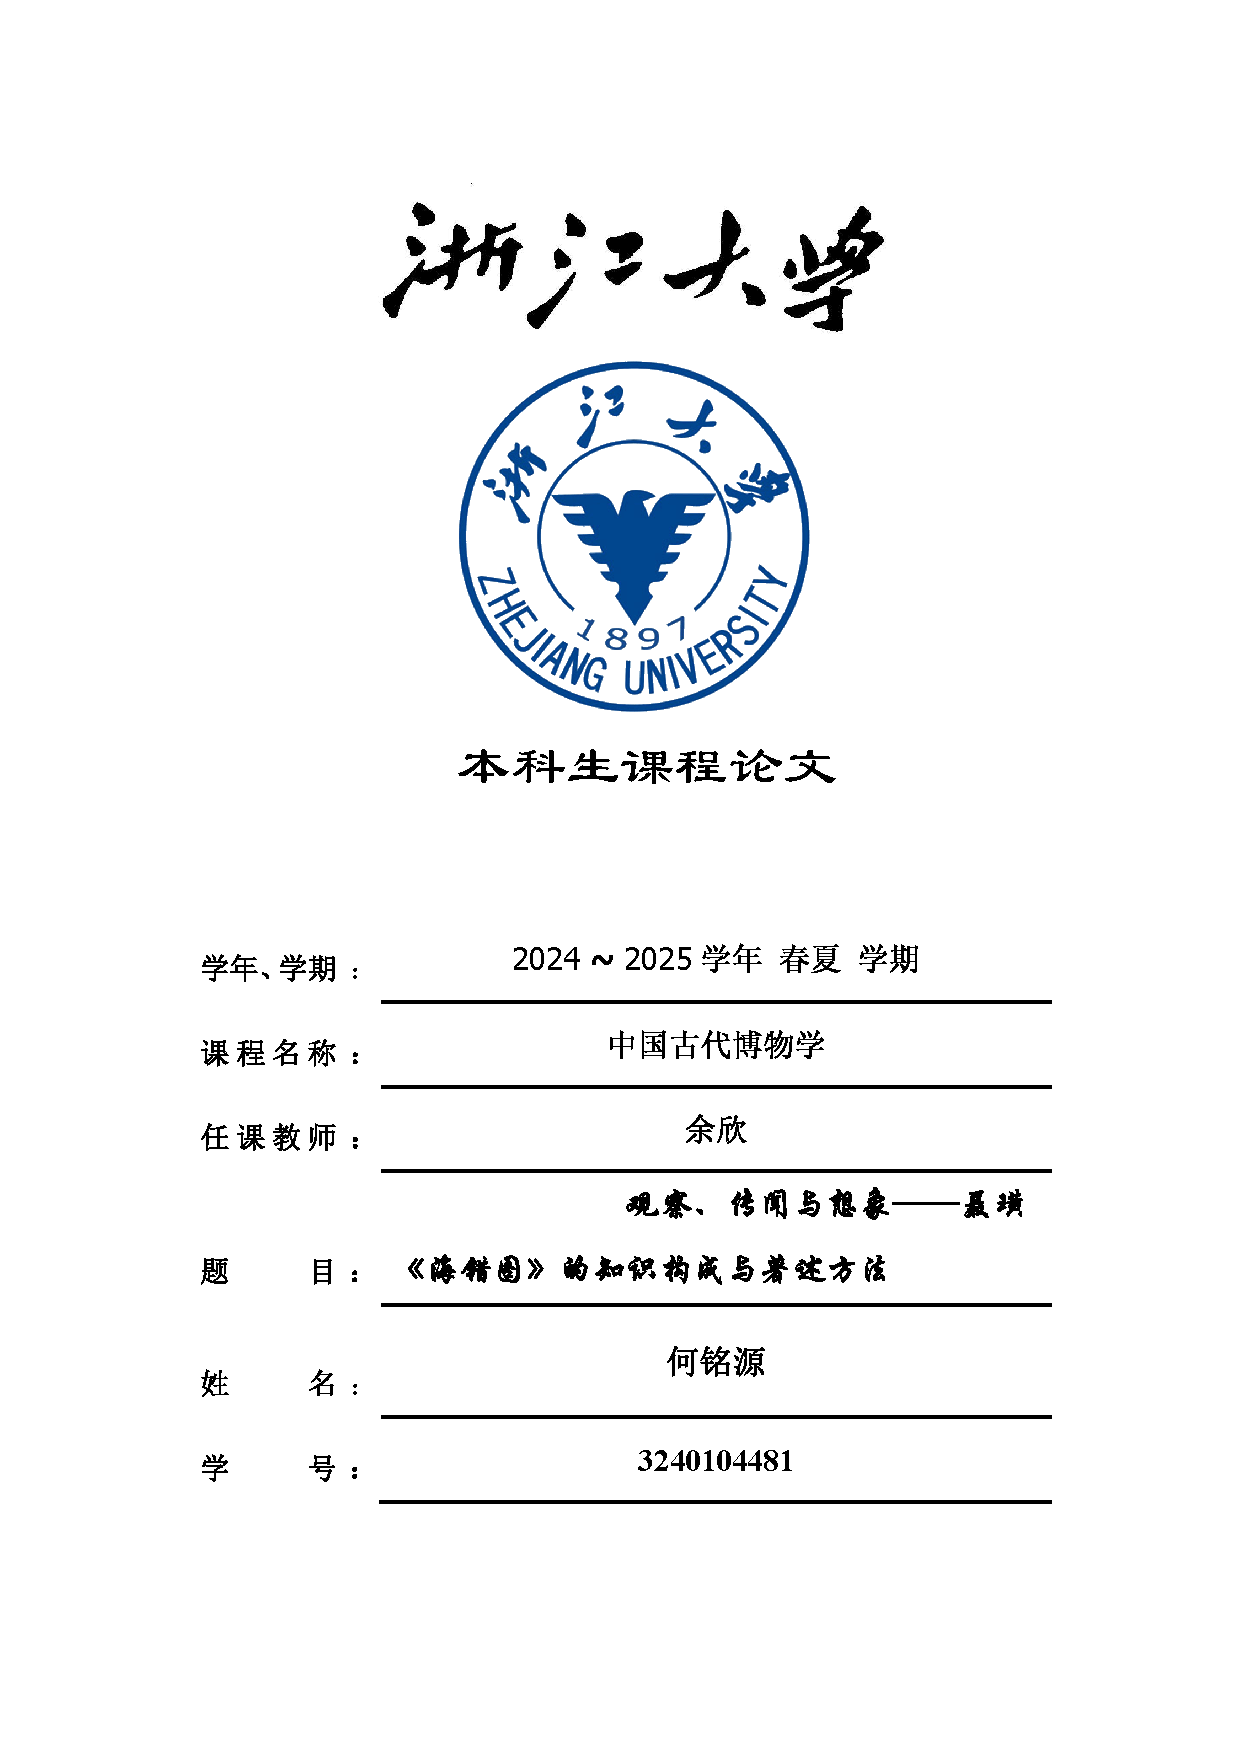
\includepdf[pages={1}]{./cover.pdf}
\makeheader
\section{引言}
\subsection{海错图简介}
清代康熙年间,一部名为《海错图》的海洋生物图谱横空出世,
成为中国古代博物学领域的一颗璀璨明珠
。此书由民间博物学爱好者聂璜历时数十年,于康熙三十七年(1698年)左右完成,
共计四册,收录了三百七十余种海洋生物及相关物事。\footnote{故宫博物院:《\textlangle 海错图\textrangle ——清代的纸上“海洋馆”》, https://young.dpm.org.cn/info/461,\today}所谓“海错”,取自古语,意指海洋中种类繁多、错综复杂的生物与物产。

聂璜,字存庵,浙江钱塘(今杭州)人,
是一位活跃于明末清初的画家及生物学爱好者。他并非科举出身的士大夫,却凭借对海洋世界的浓厚兴趣与不懈探索,
游历中国东南沿海各地,亲身观察、多方询访、考证典籍,最终将所见所闻汇集成这部图文并茂的巨著。

《海错图》的流传经历颇具传奇色彩。这部源自民间的创作,
在雍正年间由太监苏培盛带入宫中,深得清朝历代帝王,
尤其是乾隆皇帝的喜爱与重视。乾隆帝不仅命人重新装裱,
钤上“乾隆御览之宝”、“重华宫鉴藏宝”等御玺,还将其著录于《石渠宝笈续编》,
彰显了其在清宫收藏中的重要地位。
这种从民间创作到皇家珍藏的历程,凸显了《海错图》独特的价值,
它不仅是聂璜个人求知热情的结晶,也反映了清代上层社会对自然知识与精细图谱的兴趣与吸纳,成为连接民间智慧与宫廷文化的桥梁。
\subsection{学术史回顾}
\subsubsection{生物考证和科学价值}
以张辰亮《海错图笔记》系列为代表的著作,从现代生物学的角度对图中的生物进行了细致的考证和鉴定,辨识了大量物种,并指出了聂璜在认知上的一些时代局限性。
杨德渐、徐奎栋主编的《\textlangle 海错图\textrangle 通考》则是一部更为系统和全面的学术考释著作,不仅对《海错图》原文进行注释,还基于现代生物分类学研究校正了其中的错误,并引用大量古籍和现代文献考订物种的中英文及拉丁名称、形态特征、生态习性等。
\subsubsection{文化内涵与中西交流}
邹振环的研究尤为关注《海错图》在中西知识交流背景下的意义。
他指出聂璜在著作中引用了如艾儒略《职方外纪》、《西方答问》以及《西洋怪鱼图》等汉文西学文献,这表明聂璜并非完全封闭于本土知识体系,而是对西方传入的知识有所涉猎和甄别。
\subsubsection{以往研究的视阈局限与本文的切入点}
以上的学者均对海错图的科学文化方面有着深入翔实的研究,然而,对于聂璜如何具体地融合“亲眼所见、亲耳所闻”与个人想象,以及这些不同来源的信息如何在他的知识体系中互动和呈现,以往的研究虽有提及,但缺乏系统性的深入剖析。

本文的创新点正在于弥补这一不足,聚焦于聂璜《海错图》的知识来源及其多元的写作手法。通过对图中典型案例的分析,本研究旨在揭示聂璜是如何将实地考察获得的直接经验、从渔民和地方文献中收集的传闻,以及基于文化传统和个人理解的想象这三者交织融合,从而构建出其独特的十七世纪海洋知识图景。
\section{聂璜的知识探寻:来源、方法与视野}
\subsection{经验与博学的融合}
聂璜的《海错图》并非书斋中的空想之作,而是其数十年如一日辛勤付出的成果。
他“历经几十年,访遍全国各地江海湖泊,考察积累,绘制而成”,其足迹遍及河北、天津、浙江、福建等沿海地区。\footnote{苏义:《\textlangle 海错图\textrangle 大清朝的“海鲜”图鉴》,《博物》,2015年第07期}
这种深入实地的考察构成了他知识来源的基石,他强调“亲眼所见、亲耳所闻”,力求描绘的真实性。

除了亲身观察,聂璜非常重视向当地居民,尤其是渔民和海客学习。
他“每看到一种新的海洋生物,就画下来,并查阅相关的资料,或去请教当地的渔民”。
这种对地方性知识和口头传统的尊重与采纳,
使得《海错图》不仅记录了生物形态,还融入了丰富的民俗信息和实践经验。

同时,聂璜并非罔顾前人成果。
他广泛涉猎古代典籍,如《山海经》、《广东新语》等,
并将自己的观察与文献记载进行比对考证。值得注意的是,
他还接触并引用了一些受到西方知识影响的汉文著作,如《西洋怪鱼图》和艾儒略的《西方答问》。\footnote{邹振环:《清代动物图谱与中西文化交流 ——以\textlangle 兽谱\textrangle \textlangle 海错图\textrangle 为中心》,2023 年 5 月 15 日,\\http://www.ihss.pku.edu.cn/templates/learning/index.aspx?nodeid=121\&page=ContentPage\&contentid=5043,\today}
尽管他认为这些西学文献“但纪者皆外洋国族,所图者皆海洋怪鱼,于江浙闽广海滨所产无与也”,
\footnote{邹振环:《清代动物图谱与中西文化交流 ——以\textlangle 兽谱\textrangle \textlangle 海错图\textrangle 为中心》}即其内容多为域外之物,
与中国沿海生物不尽相符,但这种关注本身已显示出其开放的学术视野和试图整合不同知识来源的努力。
聂璜的治学方法,实质上是一种综合性的知识获取策略,体现了在没有严格学科划分的时代,
一位博物学爱好者如何融合个人观察、地方智慧与文献考据,构建其独特的知识体系。
这种方法可被视为一种广博探索。

\subsection{想象与传闻}
在十七、十八世纪,科学观察手段尚不发达,
人类对自然界的认知,特别是对遥远或隐秘领域的认知,
很大程度上依赖于间接信息。因此,传闻和想象在当时的知识体系中扮演着不可或缺的角色。
聂璜在《海错图》中,不仅记录“所见”,也大量采纳“所闻”。\footnote{博物:《\textlangle 海错图\textrangle 大清朝的“海鲜”图鉴》}
对于一些难以证实或超出其经验范围的生物,他会注明信息来源,甚至坦承自己的困惑,
留下“以俟后有博识者辨之”的字句。
这种做法,并非单纯的猎奇或迷信,而是在特定历史条件下,一种试图全面记录、理解复杂世界的努力。
它反映了一种求知的审慎态度:在无法亲证的情况下,忠实记录传闻,并期待后人能够进一步辨析。
这种坦诚面对知识局限性的态度,反而增强了其作品的史料价值,使我们得以窥见当时知识建构的真实过程。

\section{案例分析}
《海错图》中的生物描绘,并非整齐划一地遵循现代生物学的写实标准,而是呈现出一个从精确观察到奇幻想象的广阔光谱。
本节将选取若干典型案例,分析聂璜如何在观察、传闻与想象之间进行取舍与融合。
\subsection{观察之下的生物:可触碰的海洋世界——弹涂鱼}
聂璜笔下的“跳鱼”,即我们今天所称的弹涂鱼,是其细致观察的典范。
他对弹涂鱼的描绘,准确地捕捉了其两栖特性、栖息于滩涂以及善于跳跃、挖洞穴居的生活习性。\footnote{嘉楠:《弹涂鱼:怒目如蛙 背翅如旗》,《博物》,2016年第02期}
图谱不仅展现了生物形态,还记录了浙江宁波一带渔民利用竹筒诱捕弹涂鱼的方法,据说此法至今仍在沿用。
这部分内容,充分显示了聂璜基于直接观察和对地方习俗的了解,其记录兼具博物学和一定的民族动物学价值。
对这类常见沿海生物的准确记述,奠定了《海错图》一定的科学基础。
\begin{figure}[H]
    \centering
    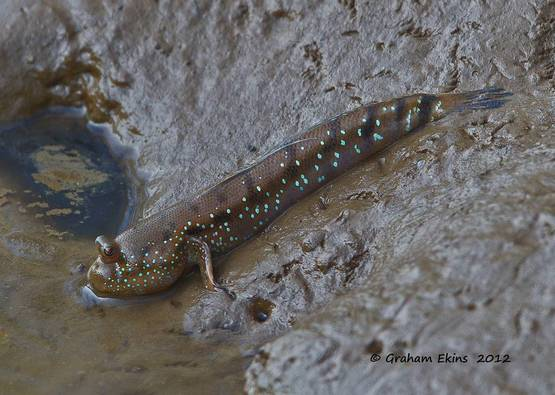
\includegraphics[width=0.8\textwidth]{fig/弹涂鱼.jpg}
    \caption{聂璜笔下的弹涂鱼~~~图片:Graham Ekins / Flickr}
    \label{fig:弹涂鱼}
\end{figure}
\subsection{传闻中的生物:被转述的知识与解读——鳄鱼}
与弹涂鱼不同,聂璜并未亲眼见过鳄鱼。
他关于鳄鱼的图文,主要依据福建人俞伯谨的口述。\footnote{何大江:《神奇动物在海里》,《成都日报》,2023 年 9 月 4 日}
俞伯谨描述的鳄鱼“口方而阔,身披厚甲,四足短而有爪,尾又长又扁”,甚至提及鳄鱼的眼、腿部有“白底衬红的火焰”。聂璜据此描绘,并因“火焰”之说而推测鳄鱼“可知鳄鱼即为龙种”。
现代学者张辰亮根据聂璜记录的鳄鱼尺寸(俞伯谨所见者“长二丈余”,约6米)和“口方而阔”等特征,推断其原型更可能是咸水鳄,
而非《海错图》后世考证所称的吻部细长的马来鳄。\footnote{张辰亮:《一席演讲:海错图笔记》,2016年 3 月 6 日,https://www.yixi.tv/h5/speech/279/,\today}

此案例清晰地展示了传闻在知识传递中的作用以及信息在转述和解读过程中可能发生的变形与增饰。
“火焰”的细节,无疑是传闻中的想象成分,而聂璜将其与“龙”联系起来,则反映了其试图将新知识纳入既有文化框架的努力。
\subsection{想象与神话的生物:奇幻的领域——人鱼}
《海错图》中对“人鱼”的描绘极具特色:“其长如人,肉黑发黄,手足、眉目、口鼻皆具,阴阳亦与男女同。
惟背有翅,红色,后有短尾及胼指,与人稍异耳。”\footnote{陈茜:《海错图》,《新华日报》,2020 年 11 月 6 日}
聂璜最初对他人提供的人鱼图像表示怀疑,但在查阅了《职方外纪》、《正字通》等文献后,才将其收入图中。
其造型奇特,近乎一个背部长着红色翅膀的秃顶中年男子。
这一个人鱼形象融合了中国本土的精怪传说(如《山海经》中的记载),
可能也受到了外来文化(如通过《职方外纪》等汉文西书传入的西方人鱼概念)的影响。
学者邹振环便在《海错图》的人鱼中看到了中西知识交流的痕迹。\footnote{邹振环:《清代动物图谱与中西文化交流 ——以\textlangle 兽谱\textrangle \textlangle 海错图\textrangle 为中心》}
张辰亮则指出,并非所有地区的人鱼传说都起源于儒艮,尤其是在儒艮分布范围之外的欧洲。\footnote{张辰亮:《海错图笔记》,北京:中信出版社,2016年,第111页}
人鱼的案例表明,聂璜在处理这类充满神秘色彩的生物时,会试图寻求文献佐证,其知识构建是在既有文化资源和新信息来源的互动中完成的。
\begin{figure}[H]
    \centering
    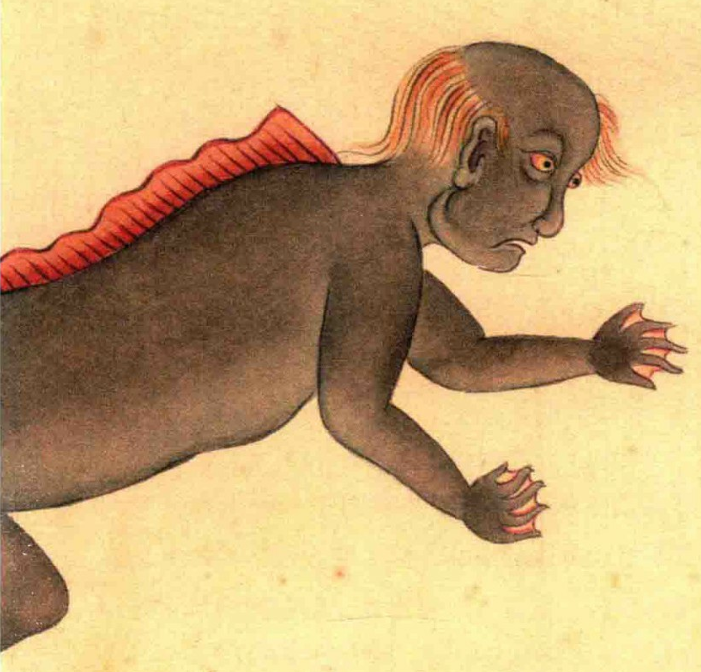
\includegraphics[width=0.8\textwidth]{fig/人鱼.png}
    \caption{聂璜笔下的人鱼~~~图片:张辰亮}
    \label{fig:人鱼}
\end{figure}
\subsection{模糊界限的生物:观察、解读与想象的交织——井鱼}
“井鱼”的记载,则巧妙地融合了观察、传闻与想象。
聂璜描述其“头上有一穴,贮水冲起,多在大洋”。
船员常常见到,并传说其喷出的水经过脑穴后会由咸变淡,可供饮用。\footnote{邹振环:《略说海错图》,《紫禁城》,2017年第03期}
他还引用了《汇苑》、《四译考》以及《西方答问》中关于类似喷水巨兽的记载,后者描述了西方海域中头有两角、能喷水沉舟的大鱼。
井鱼的形象,很可能源于对鲸类喷水行为的观察,但其喷出淡水的神奇特性,则属于传闻和想象的范畴。
聂璜旁征博引,试图通过中外文献来理解这一现象,正体现了他在面对奇异现象时,整合多种信息来源进行“合理化”解释的努力。
\subsection{总结}
通过这些案例可见,《海错图》中的生物并非简单地划分为“真实”与“虚构”。
许多条目都处在一个连续的光谱之上,反映了聂璜在构建其海洋知识体系时,对经验材料、文化先验观念和叙事传统的复杂协商。
十七世纪的观察条件有限,尤其对于广阔而神秘的海洋,直接观察难以覆盖所有生物,这自然导致对传闻的依赖,并为想象力留下了广阔的空间。
聂璜将实用信息(如弹涂鱼的捕捞、海产的烹饪)与奇闻怪谈并置一处,
表明其意在汇集广义上的“海错”知识,既包括其实用价值,
也涵括其文化意涵与引人入胜的神秘色彩。
这种包容性,正是《海错图》作为一部反映十七世纪中国民间博物学思想的珍贵文献的关键所在。
它不仅记录了当时人们对海洋生物的认知水平,更重要的是,它揭示了那个时代人们如何看待、
理解和想象他们赖以生存又充满未知的海洋世界。
\section{《海错图》的多元价值:艺术成就、文化史料与博物学探索}
\subsection{艺术价值与风格独特性}
《海错图》不仅是一部博物图志,亦是一件具有高度艺术价值的作品。
聂璜的绘画风格细腻生动,色彩鲜艳,构图独具匠心。
他笔下的海洋生物,无论是写实的鱼虾,还是奇幻的怪兽,都栩栩如生,跃然纸上。
其画风融合了中国传统工笔画的细致与民间艺术的活泼,部分描绘的写实性,如对锯鲨的刻画,甚至被认为可能受到了西方博物画的影响。
然而,聂璜并未完全囿于写实,其作品中时常流露出一种“卡通化”的趣味和生动的神态,
这使得《海错图》在视觉上极富吸引力,迥异于纯粹的科学插图或纯粹的幻想画作。

尤为重要的是其“图文并茂”的编排形式。
每一幅图画都配有聂璜的文字描述,内容不仅包括生物的产地、习性、外貌特征,还常常附有相关的传说故事、民间歌谣,
乃至作者亲自撰写的赞美诗。
这种图像与文本的紧密结合,使得《海错图》超越了一般画谱的范畴,成为一部集知识性、趣味性和文学性于一体的综合性作品。
\subsection{对理解清代海洋认知与民间知识的贡献}
《海错图》为我们理解十七、十八世纪中国社会,特别是沿海地区民众如何认知海洋环境及其生物,提供了极为珍贵的视角。
它不仅反映了当时博物学的水平,更重要的是,它保存了大量关于海洋的民间信仰、传说故事以及与海洋相关的实用知识,如捕鱼技巧、海产烹饪方法等。
这些内容往往是正统史书和官方文献所忽略的,却生动地再现了当时沿海社会的文化生态和民众生活。

聂璜作为一位“民间博物学高手”,
其创作自由度相对较大,不像宫廷画家那样受到严格的题材和风格限制。
这种身份使其能够更广泛地接触和采纳来自民间的多元信息,包括渔民的经验之谈、地方的奇闻异事等。
因此,《海错图》在某种程度上可以被视为一部“海洋民俗志”,记录了当时民众眼中丰富多彩、既真实又充满想象的海洋世界。
\subsection{《海错图》在中西科技文化交流背景下的意义}
尽管聂璜主要关注中国本土的海洋生物,但他对一些汉文西学文献的涉猎,如《西洋怪鱼图》、《西方答问》等,表明他并非完全封闭于本土知识体系之内。
他能够注意到这些外来知识,并进行一定的比较和评判(如认为其所述多为远洋异物),这本身就反映了清初一部分知识人对“西学”的某种程度的开放态度和批判性吸收。

《海错图》的这一面向,使其成为研究早期中西知识交流史的一个有趣案例。
它展示了在精英阶层的宫廷与传教士互动之外,西学知识如何以文献的形式在民间流传,并被像聂璜这样的个体知识分子所接触和认知。
虽然这种影响可能尚不深入,但《海错图》无疑为我们理解那个时代知识构成的多元性和复杂性提供了佐证。
\subsection{现代重估与意义}
历经数百年沉寂后,《海错图》在当代重新焕发了生机。故宫博物院等机构的整理出版,\footnote{马顺平:《\textlangle 海错图 \textrangle 在清宫》,《紫禁城》,2025年05期}
以及张辰亮《海错图笔记》等大众科普读物的广泛传播,使得这部古老的图谱重新进入公众视野,并引发了广泛的兴趣。
这些现代的解读和传播,不仅让更多人领略到《海错图》的艺术魅力和奇趣内容,也推动了对其学术价值的深入研究。

以《〈海错图〉通考》为代表的学术著作,从现代生物学、文献学、文化史等多个角度对《海错图》进行了系统的注释、考订和研究。
这些研究不仅辨识了图谱中的物种(据称82.6\%的物种可鉴定至科、属、种\footnote{何大江:《神奇动物在海里》}),
订正了聂璜的一些认知错误,更发掘了其在科学史、艺术史和文化史上的多重价值。这种现代的“再发现”,
反映了当代社会对传统文化中蕴含的博物智慧、艺术创造以及人与自然互动历史的重新珍视。
人们不仅惊叹于聂璜的细致观察和生动描绘,更着迷于他那个时代独特的认知方式——一种科学精神、人文关怀与艺术想象力交织的博物世界观。
\section{结论:透过十七世纪之眼看海洋}
《海错图》不仅是一部精美的海洋生物图谱,
更是一面镜子,映照出十七世纪中国一位民间博物学爱好者是如何在观察、传闻与想象的张力中构建其对海洋世界的认知的。
它雄辩地证明了在那个特定的历史语境下,经验探究、文化叙事与艺术再现是如何紧密交织,共同塑造了人们对自然界的理解。

《海错图》的价值,远不止于其对部分海洋生物的描绘。
更深远的意义在于,它整体呈现了前现代社会对海洋这一既提供丰饶物产又蕴藏无尽神秘的广阔空间的一种整体性认知。
这种认知是生态的、文化的,也是充满敬畏与好奇的。
聂璜以一己之力,历时数十载,试图将他所能触及的关于“海错”的一切——真实的、传说的、实用的、奇妙的——尽数收录笔下,
这本身就是一种宏大的“世界构建”行为。他虽在完成此书后“消失在民间”,
但其心血凝结的《海错图》却得以流传,成为一座连接古今的桥梁,让我们得以窥见古人眼中那片既熟悉又陌生的海洋。
\end{document}